\documentclass[tikz,border=6pt]{standalone}
\usepackage{amsmath}
\colorlet{cG}{teal!70!black}
\colorlet{cO}{orange!85!black}
\newcommand{\fbar}[4]{% x, h0, h1, colour
  \fill[#4!85!white] (#1,#2) rectangle (#1+0.62,#3);
  \fill[#4!55!black] (#1+0.62,#2) -- (#1+0.84,#2+0.16) -- (#1+0.84,#3+0.16) -- (#1+0.62,#3) -- cycle;
  \fill[#4!35!white] (#1,#3) -- (#1+0.62,#3) -- (#1+0.84,#3+0.16) -- (#1+0.22,#3+0.16) -- cycle;
  \draw[black!55,line width=0.25pt] (#1,#2) rectangle (#1+0.62,#3);}
\begin{document}
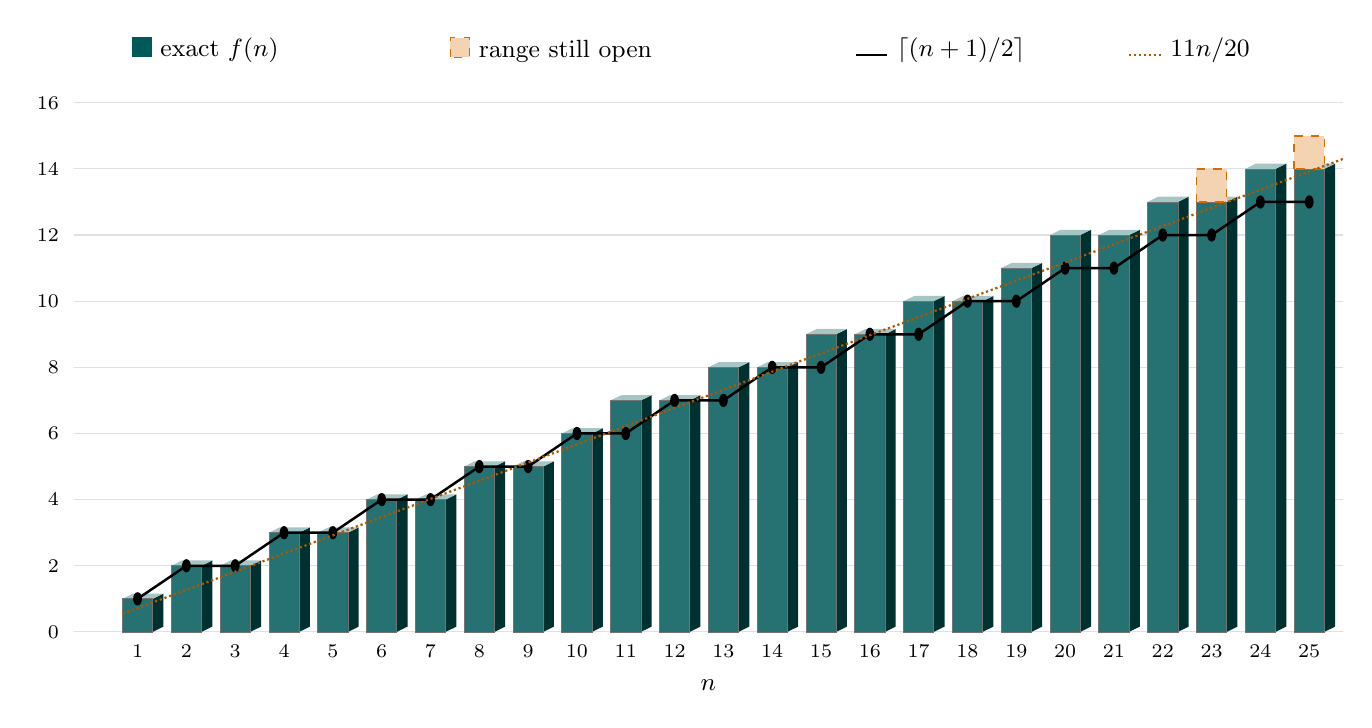
\begin{tikzpicture}[yscale=0.42,xscale=0.62]
\foreach \y in {0,2,...,16}{\draw[black!12] (0,\y) -- (26,\y); \node[font=\scriptsize,anchor=east] at (-0.1,\y) {\y};}
\fbar{1}{0}{1}{cG}
\node[font=\scriptsize] at (1+0.31,-0.6) {1};
\fbar{2}{0}{2}{cG}
\node[font=\scriptsize] at (2+0.31,-0.6) {2};
\fbar{3}{0}{2}{cG}
\node[font=\scriptsize] at (3+0.31,-0.6) {3};
\fbar{4}{0}{3}{cG}
\node[font=\scriptsize] at (4+0.31,-0.6) {4};
\fbar{5}{0}{3}{cG}
\node[font=\scriptsize] at (5+0.31,-0.6) {5};
\fbar{6}{0}{4}{cG}
\node[font=\scriptsize] at (6+0.31,-0.6) {6};
\fbar{7}{0}{4}{cG}
\node[font=\scriptsize] at (7+0.31,-0.6) {7};
\fbar{8}{0}{5}{cG}
\node[font=\scriptsize] at (8+0.31,-0.6) {8};
\fbar{9}{0}{5}{cG}
\node[font=\scriptsize] at (9+0.31,-0.6) {9};
\fbar{10}{0}{6}{cG}
\node[font=\scriptsize] at (10+0.31,-0.6) {10};
\fbar{11}{0}{7}{cG}
\node[font=\scriptsize] at (11+0.31,-0.6) {11};
\fbar{12}{0}{7}{cG}
\node[font=\scriptsize] at (12+0.31,-0.6) {12};
\fbar{13}{0}{8}{cG}
\node[font=\scriptsize] at (13+0.31,-0.6) {13};
\fbar{14}{0}{8}{cG}
\node[font=\scriptsize] at (14+0.31,-0.6) {14};
\fbar{15}{0}{9}{cG}
\node[font=\scriptsize] at (15+0.31,-0.6) {15};
\fbar{16}{0}{9}{cG}
\node[font=\scriptsize] at (16+0.31,-0.6) {16};
\fbar{17}{0}{10}{cG}
\node[font=\scriptsize] at (17+0.31,-0.6) {17};
\fbar{18}{0}{10}{cG}
\node[font=\scriptsize] at (18+0.31,-0.6) {18};
\fbar{19}{0}{11}{cG}
\node[font=\scriptsize] at (19+0.31,-0.6) {19};
\fbar{20}{0}{12}{cG}
\node[font=\scriptsize] at (20+0.31,-0.6) {20};
\fbar{21}{0}{12}{cG}
\node[font=\scriptsize] at (21+0.31,-0.6) {21};
\fbar{22}{0}{13}{cG}
\node[font=\scriptsize] at (22+0.31,-0.6) {22};
\fbar{23}{0}{13}{cG}
\fill[cO!30!white] (23,13) rectangle (23+0.62,14); \draw[cO,dashed,line width=0.5pt] (23,13) rectangle (23+0.62,14);
\node[font=\scriptsize] at (23+0.31,-0.6) {23};
\fbar{24}{0}{14}{cG}
\node[font=\scriptsize] at (24+0.31,-0.6) {24};
\fbar{25}{0}{14}{cG}
\fill[cO!30!white] (25,14) rectangle (25+0.62,15); \draw[cO,dashed,line width=0.5pt] (25,14) rectangle (25+0.62,15);
\node[font=\scriptsize] at (25+0.31,-0.6) {25};
\draw[black,line width=0.9pt] (1+0.31,1) -- (2+0.31,2) -- (3+0.31,2) -- (4+0.31,3) -- (5+0.31,3) -- (6+0.31,4) -- (7+0.31,4) -- (8+0.31,5) -- (9+0.31,5) -- (10+0.31,6) -- (11+0.31,6) -- (12+0.31,7) -- (13+0.31,7) -- (14+0.31,8) -- (15+0.31,8) -- (16+0.31,9) -- (17+0.31,9) -- (18+0.31,10) -- (19+0.31,10) -- (20+0.31,11) -- (21+0.31,11) -- (22+0.31,12) -- (23+0.31,12) -- (24+0.31,13) -- (25+0.31,13);
\foreach \n in {1,...,25}{\pgfmathtruncatemacro{\c}{(\n+2)/2}\fill[black] (\n+0.31,\c) circle (0.09 and 0.2);}
\draw[cO!80!black,line width=0.8pt,densely dotted] (1,0.55) -- (26,0.55*26);
\node[font=\small] at (13,-1.6) {$n$};
\node[font=\small,anchor=west] at (1,17.6) {\tikz\fill[cG] (0,0) rectangle (0.25,0.25); exact $f(n)$};
\node[font=\small,anchor=west] at (7.5,17.6) {\tikz\draw[cO,dashed,fill=cO!30!white] (0,0) rectangle (0.25,0.25); range still open};
\node[font=\small,anchor=west] at (15.8,17.6) {\tikz\draw[black,line width=0.9pt] (0,0.1)--(0.4,0.1); $\lceil (n+1)/2\rceil$};
\node[font=\small,anchor=west] at (21.4,17.6) {\tikz\draw[cO!80!black,densely dotted,line width=0.8pt] (0,0.1)--(0.4,0.1); $11n/20$};
\end{tikzpicture}
\end{document}
